\documentclass{beamer}
\newcommand\tab[1][1cm]{\hspace*{#1}}
\usepackage{tikz}
\usepackage{rotating}

\title{Load Balancing for ALICE}
\subtitle{Software for Science, CERN}

\usetheme{Berkeley}
\usecolortheme{beaver}
\begin{document}

\beamertemplatenavigationsymbolsempty
\def\logo{%
  
\includegraphics[width=2cm]{./graphics/logo.png}%
}

\setbeamertemplate{footline}{
  \begin{minipage}[t]{0.9\paperwidth}
    \hfill
    \begin{beamercolorbox}[wd=1cm, ht = 0.05cm]{page number in head/foot}
      \logo
    \end{beamercolorbox}
  \end{minipage}
}

	\frame {
		\titlepage
	}
	\frame {
		\frametitle{Index}
		\begin{itemize}
			\item Introduction
			\item ALICE
			\item Load Balancing
			\item Cluster
			\item Experiments
			
			\begin{itemize}
			\item Experiment 1
			\item Experiment 2
			\item Experiment 3
			\item Experiment 4
			\item Experiment 5
			\end{itemize}
			
			\item Conclusions
			\item Recommendations
		\end{itemize}
	}
	
	% Introduction
	\frame {
		\frametitle{Introduction}
		\begin{columns}[T]
		
		\begin{column}{0.5\textwidth}
		~\\~\\
		\begin{itemize}
			\item Mitchell Puls
			\begin{itemize}
				\item 500659986
				\item mitchpuls@upcmail.nl
				\item mitch.puls@hva.nl
				\item +31615050310
			\end{itemize}
			\item Mentor
			\begin{itemize}
				\item C.J. Rijsenbrij
			\end{itemize}
			\item Company Supervisor
			\begin{itemize}
				\item Dr. M. Teitsma
			\end{itemize}
		\end{itemize}
		\end{column}
		
		\begin{column}{0.5\textwidth}
		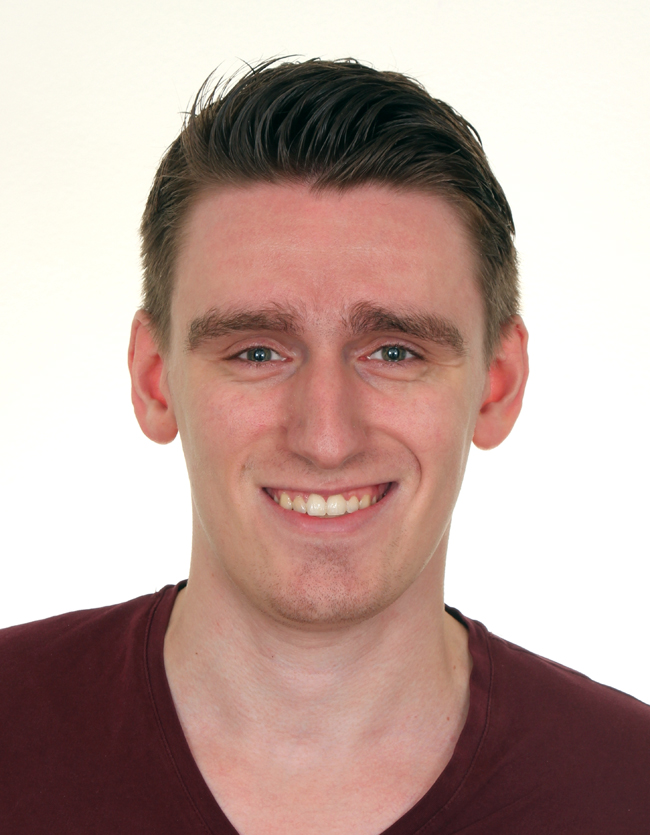
\includegraphics[scale=0.8]{./graphics/foto.jpg}
		\end{column}
		
		\end{columns}
	}
	
	% ALICE
	\frame {
		\frametitle{ALICE}
		\begin{columns}[T]
		
		\begin{column}{0.5\textwidth}
		~\\~\\~\\
		\begin{itemize}
			\item CERN
			\item LHC
			\item ALICE
		\end{itemize}
		\end{column}
		
		\begin{column}{0.5\textwidth}
		
\includegraphics[scale=0.3]{./graphics/alice.png}
		\end{column}
		
		\end{columns}
		\footnote{http://alice-collaboration.web.cern.ch/}
	}
	
	% Load Balancing
	\frame{
		\frametitle{Load Balancing}
		\begin{columns}[T]
		\begin{column}{0.5\textwidth}
		~\\~\\~\\
		\begin{itemize}
			\item Setup
			\begin{itemize}
			\item First Level Processors (FLP)
			\item Event Processing Nodes (EPN)
			\item Information Node (IN)
			\end{itemize}
			\item Blacklist Algorithm
		\end{itemize}
		\end{column}
		\begin{column}{0.5\textwidth}
		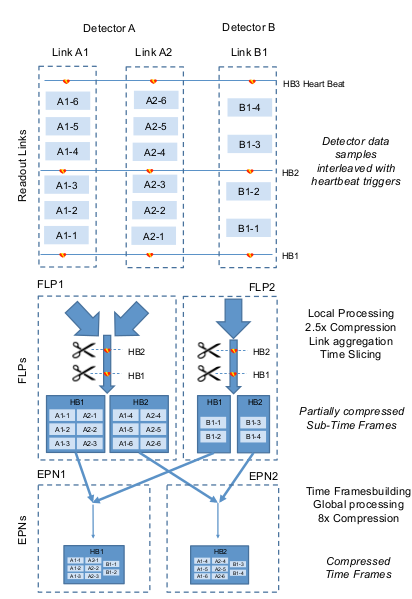
\includegraphics[scale=0.3]{./graphics/data_aggregation.png}
		\end{column}
		\end{columns}
		\footnote{Technical Design Report for the Upgrade of the Online Offline Computing System, 2015, p. 34}
	}
	
	% Cluster
	\frame{
	    \frametitle{Cluster}
	    \begin{columns}[T]
	    \begin{column}{0.5\textwidth}
		~\\~\\~\\
		\begin{itemize}
			\item Raspberry Pi
			\item Cluster
			\item 2nd Ethernet Interface
		\end{itemize}
	    \end{column}
	    \begin{column}{0.5\textwidth}
	    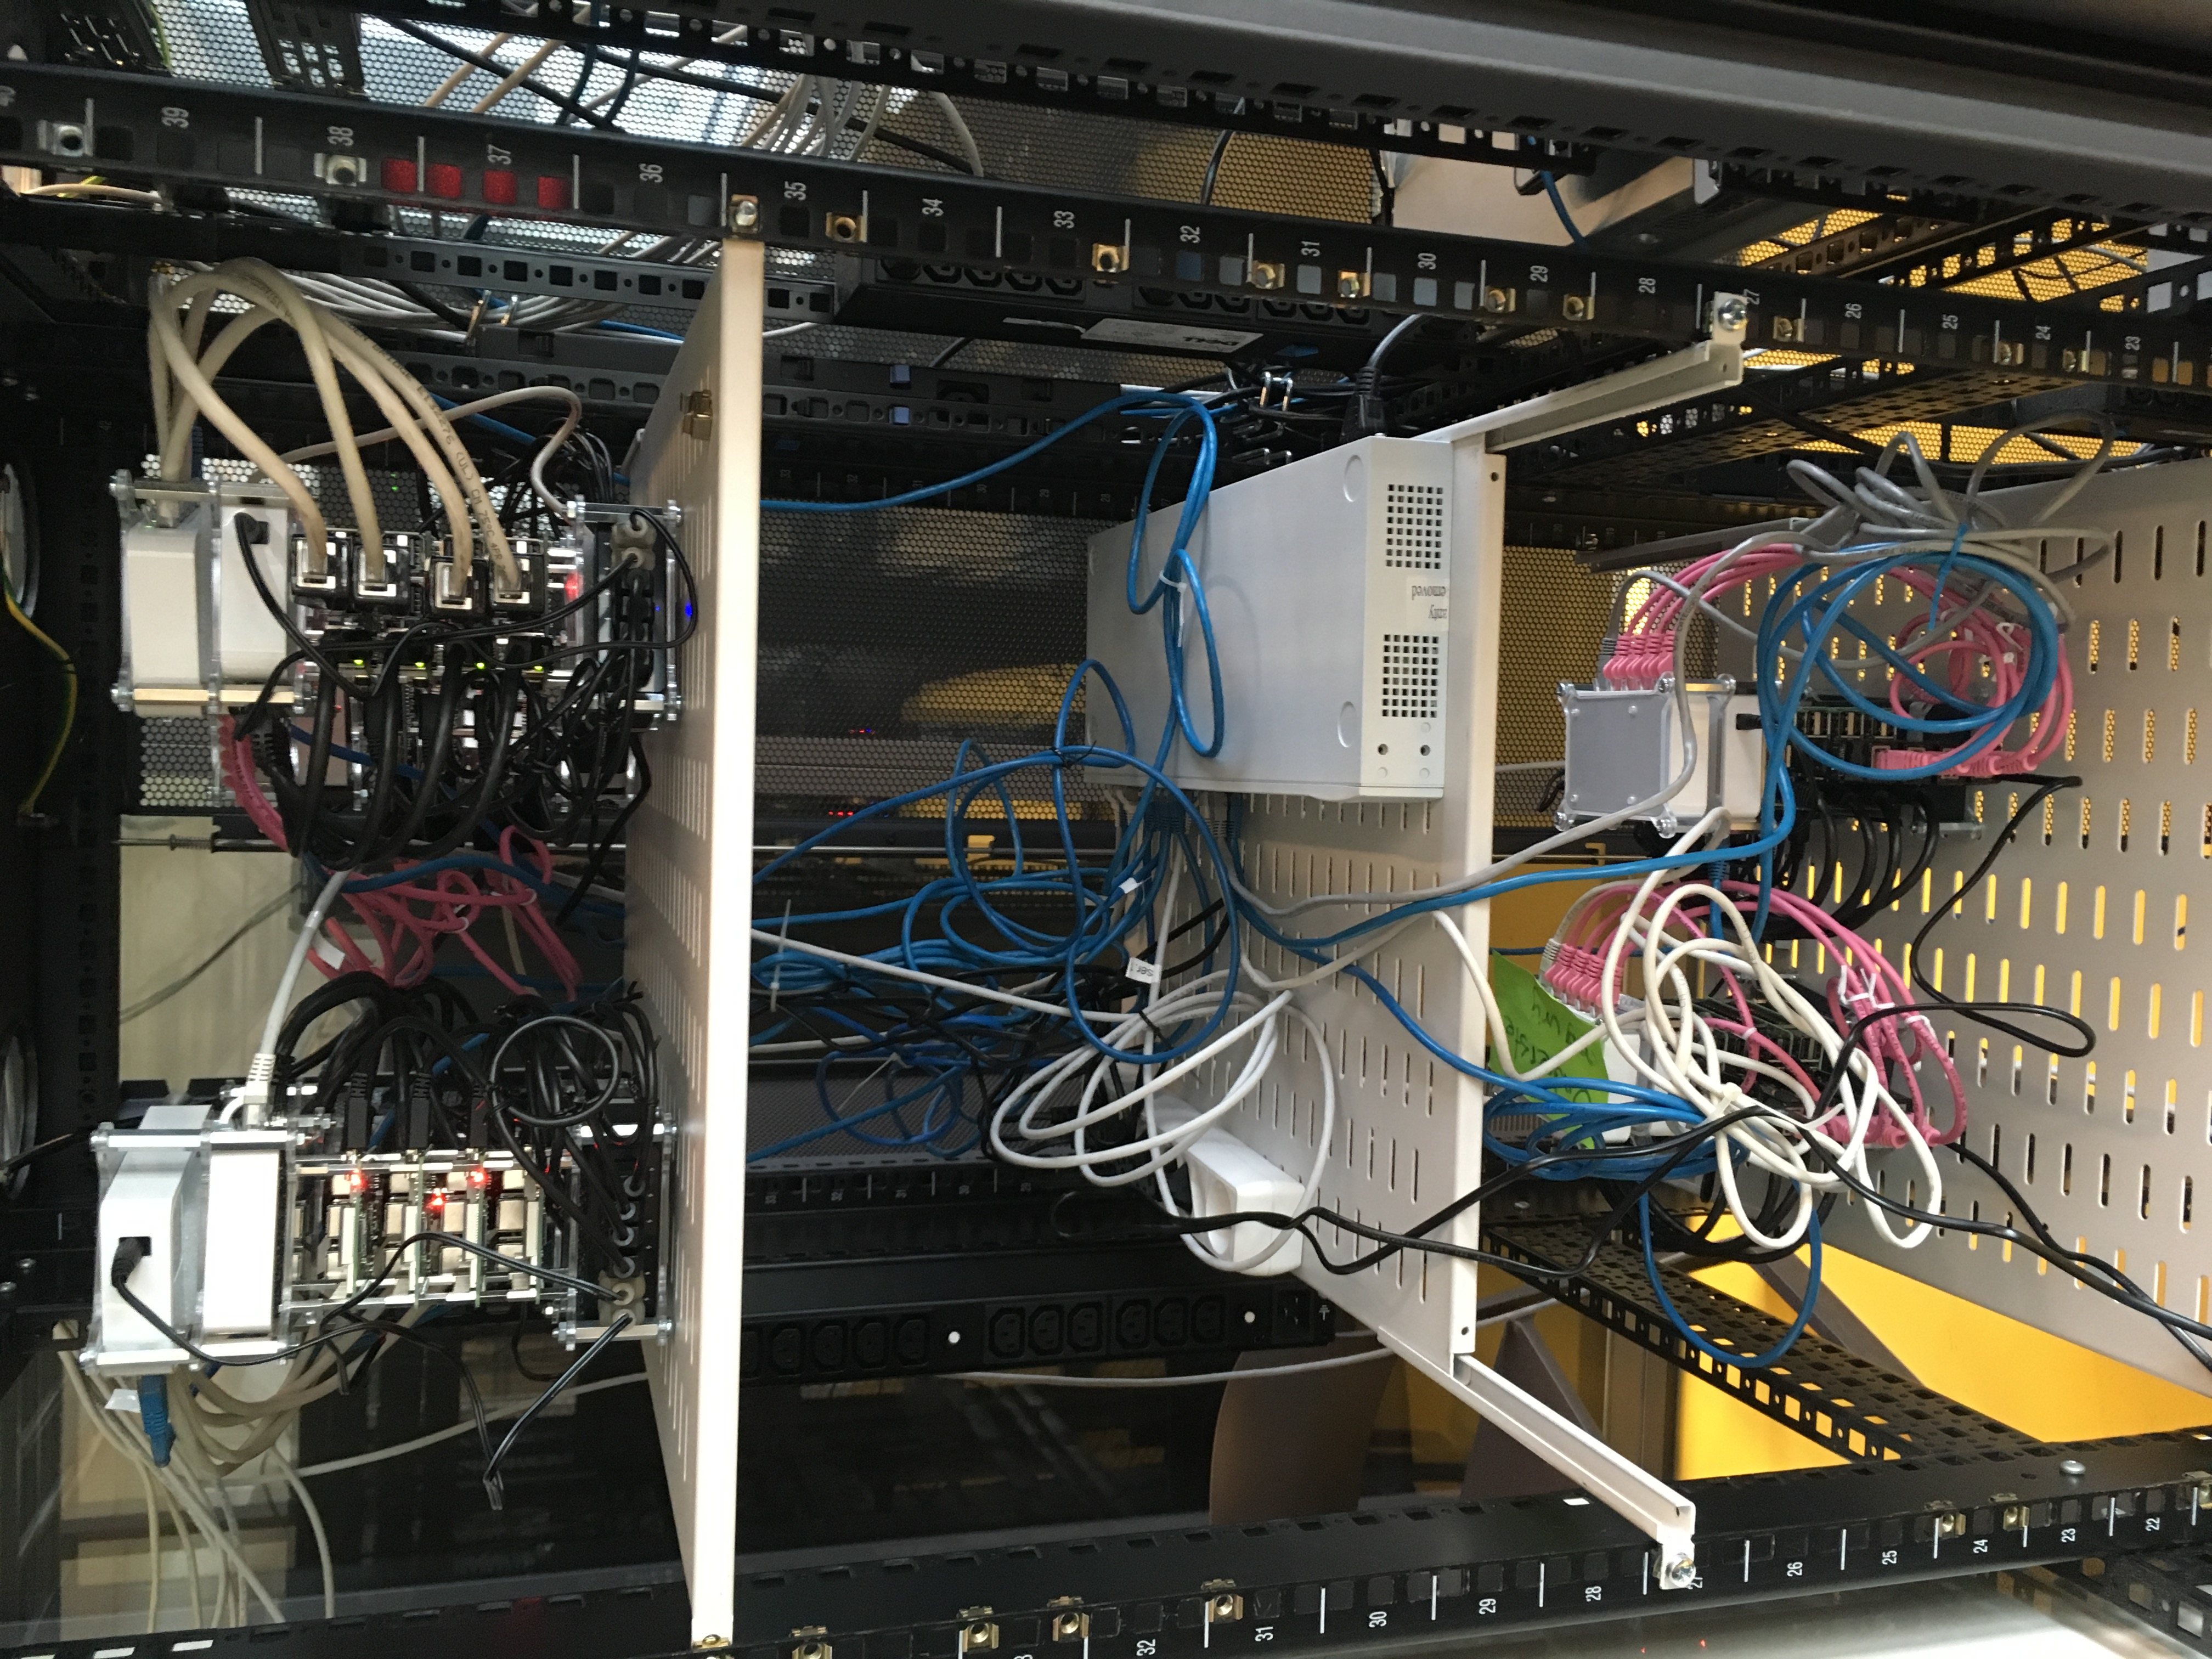
\includegraphics[angle=-90,origin=c,scale=0.04]{./graphics/cluster.JPG}
	    \end{column}
	    \end{columns}
	}
	\frame{
		\frametitle{Cluster}
		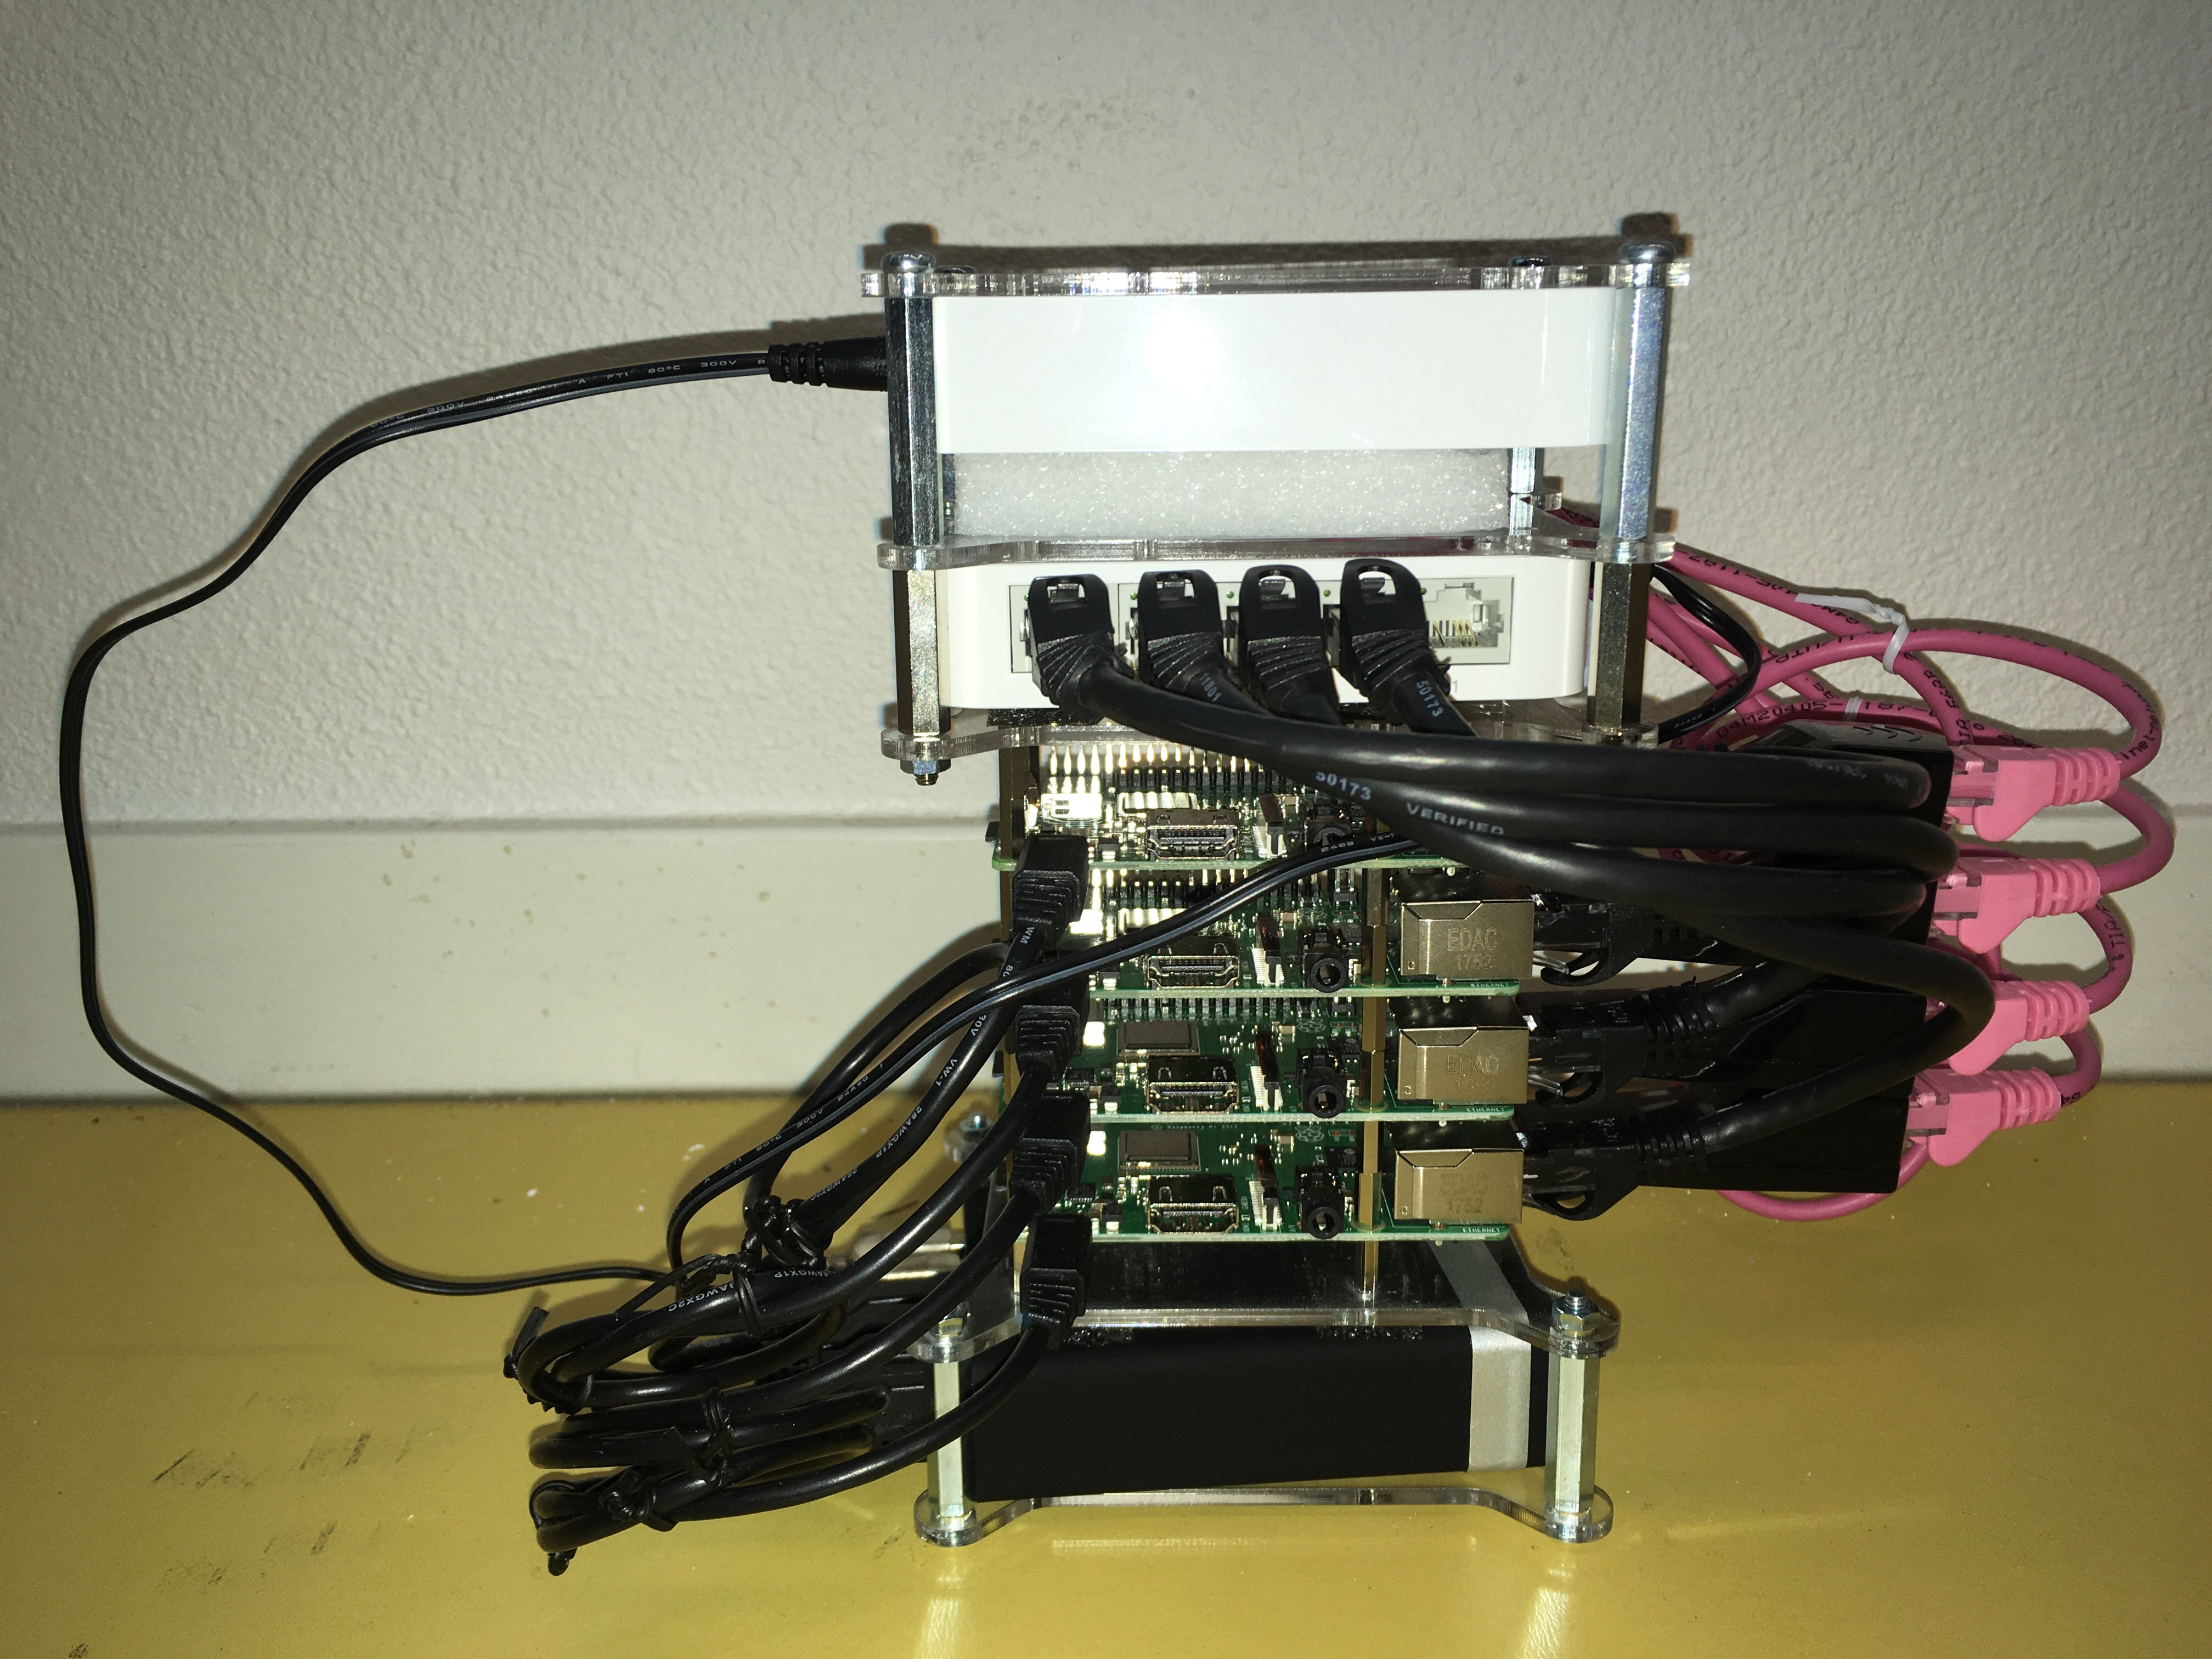
\includegraphics[scale=0.06]{./graphics/single_cluster.JPG}	
	}
	
	% Experiments
	\frame{
		\frametitle{Experiments}
		\begin{columns}[T]
		
		\begin{column}{0.3\textwidth}
		~\\~\\~\\
		\begin{itemize}
			\item Ratio
			\item Compare
			\item Expand
		\end{itemize}
		\end{column}
		
		\begin{column}{0.7\textwidth}
		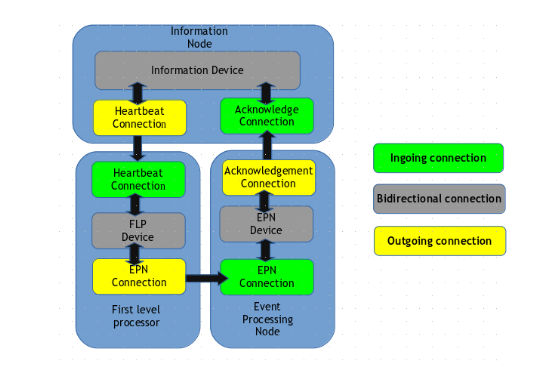
\includegraphics[scale=0.5]{./graphics/connection_diagram.png}
		\end{column}
		
		\end{columns}
		
		\footnote{Block diagram of the cluster connections (van der Heijden, 2018, p. 22)}
	}
	\frame{
		\frametitle{Experiments}
		\framesubtitle{Experiment 1}
		\begin{columns}[T]
		
		\begin{column}{0.5\textwidth}
		~\\~\\~\\
		\begin{itemize}
			\item Definition
		\end{itemize}
		Ticktime influence on the Blacklist algorithm with one fail-over
		\end{column}
		
		\begin{column}{0.5\textwidth}
		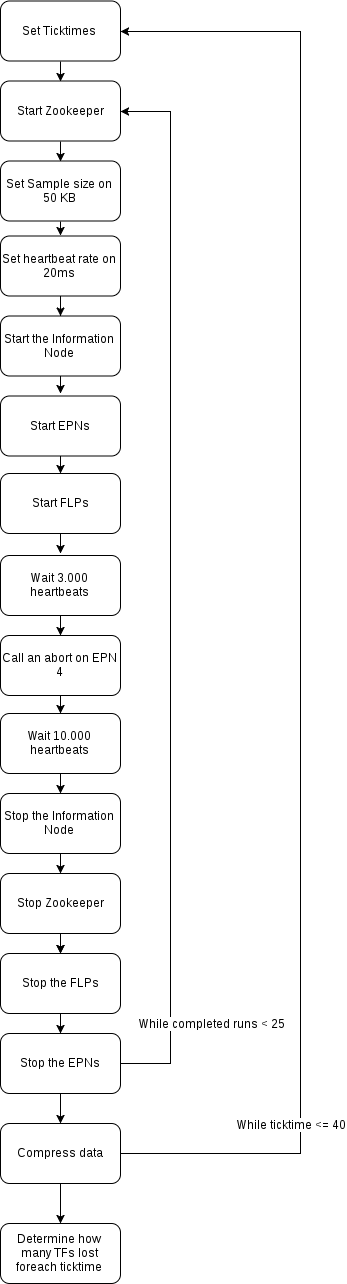
\includegraphics[scale=0.2]{./graphics/ex1.png}
		\end{column}
		
		\end{columns}
		\footnote{Effects of the EPNs and FLPs on the Information Node for ALICE (Puls, 2018, p. 21)}
	}
	\frame{
		\frametitle{Experiment 1}
		\framesubtitle{Results}
		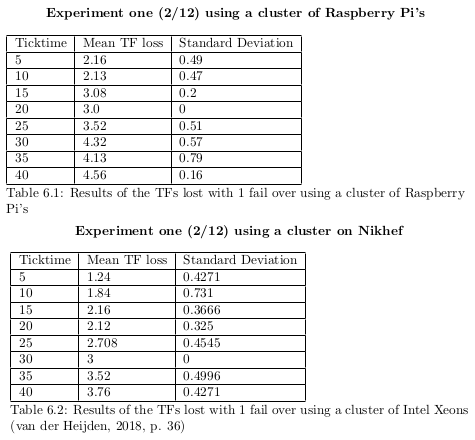
\includegraphics[scale=0.5]{./graphics/res1.png}
	}
	\frame{
		\frametitle{Experiment 1}
		\framesubtitle{Results}
		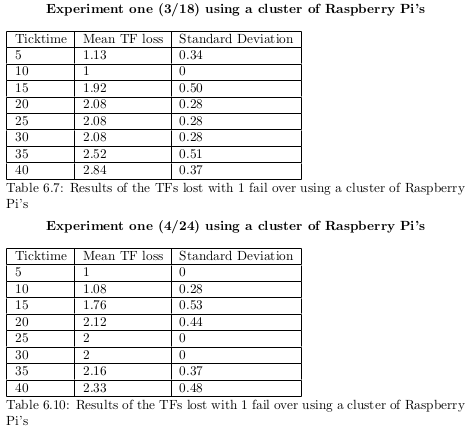
\includegraphics[scale=0.5]{./graphics/res1ex.png}
	}
	\frame{
		\frametitle{Experiments}
		\framesubtitle{Experiment 2}
		\begin{columns}[T]
		
		\begin{column}{0.5\textwidth}
		~\\~\\~\\
		\begin{itemize}
			\item Definition
		\end{itemize}
		Ticktime influence on the Blacklist algorithm with all but one fail-over
		\end{column}
		
		\begin{column}{0.5\textwidth}
		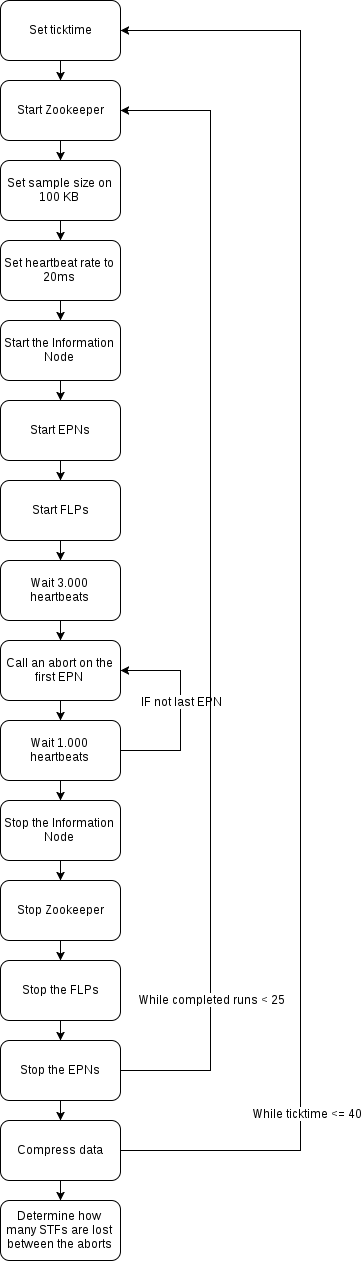
\includegraphics[scale=0.2]{./graphics/ex2.png}
		\end{column}
		
		\end{columns}
		\footnote{Effects of the EPNs and FLPs on the Information Node for ALICE (Puls, 2018, p. 23)}
	}
	\frame{
		\frametitle{Experiment 2}
		\framesubtitle{Results}
		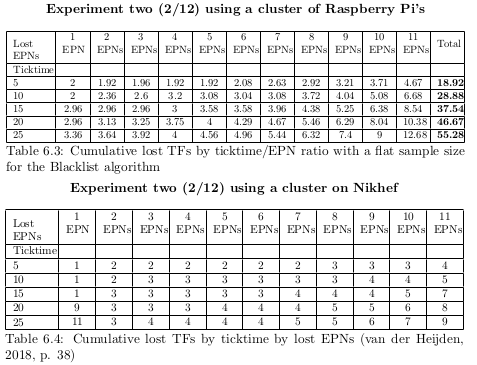
\includegraphics[scale=0.5]{./graphics/res2.png}
	}
	\frame{
		\frametitle{Experiment 2}
		\framesubtitle{Results}
		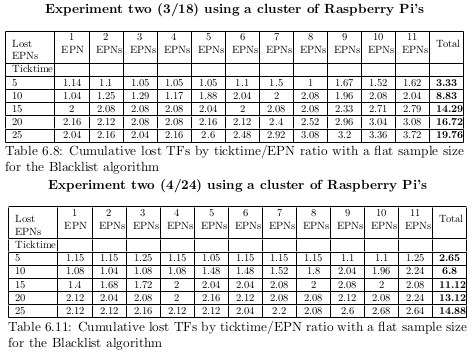
\includegraphics[scale=0.5]{./graphics/res2ex.png}
	}
	\frame{
		\frametitle{Experiments}
		\framesubtitle{Experiment 3}
		\begin{columns}[T]
		
		\begin{column}{0.5\textwidth}
		~\\~\\~\\
		\begin{itemize}
			\item Definition
		\end{itemize}
		Ticktime influence on the Blacklist algorithm with all but one fail-over using a random sample size
		\end{column}
		
		\begin{column}{0.5\textwidth}
		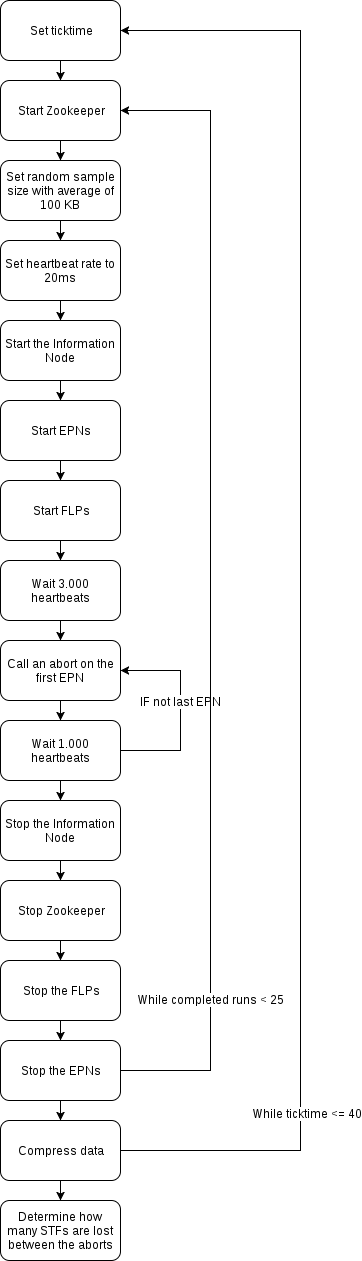
\includegraphics[scale=0.2]{./graphics/ex3.png}
		\end{column}
		
		\end{columns}		
		\footnote{Effects of the EPNs and FLPs on the Information Node for ALICE (Puls, 2018, p. 24)}
	}
	\frame{
		\frametitle{Experiment 3}
		\framesubtitle{Results}
		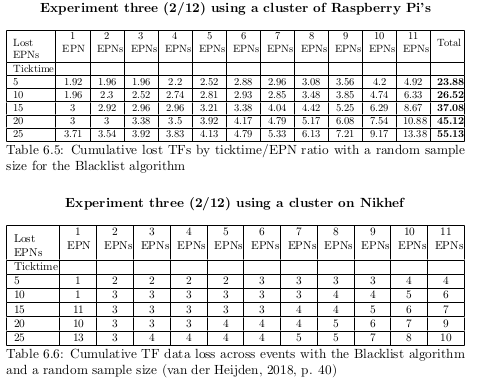
\includegraphics[scale=0.5]{./graphics/res3.png}
	}
	\frame{
		\frametitle{Experiment 3}
		\framesubtitle{Results}
		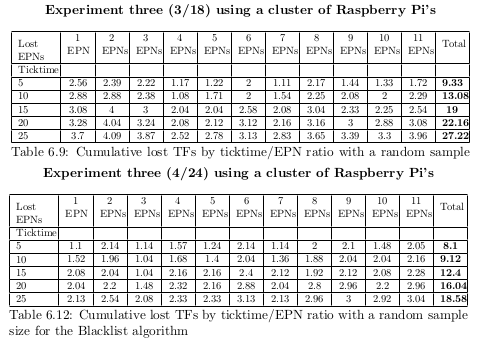
\includegraphics[scale=0.5]{./graphics/res3ex.png}
	}
	\frame{
		\frametitle{Experiments}
		\framesubtitle{Experiment 4}
		\begin{columns}[T]
		
		\begin{column}{0.5\textwidth}
		~\\~\\~\\
		\begin{itemize}
			\item Definition
		\end{itemize}
		Ticktime influence on the Blacklist algorithm with a fixed cluster fail-over pattern using a random sample size
		\end{column}
		
		\begin{column}{0.5\textwidth}
		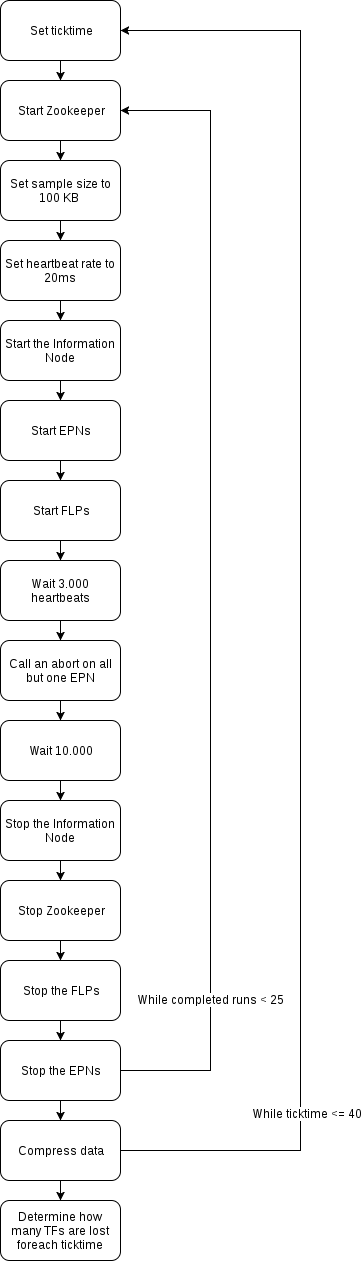
\includegraphics[scale=0.2]{./graphics/ex4.png}
		\end{column}
		
		\end{columns}
		\footnote{Effects of the EPNs and FLPs on the Information Node for ALICE (Puls, 2018, p. 25)}
	}
	\frame{
		\frametitle{Experiment 4}
		\framesubtitle{Results}
		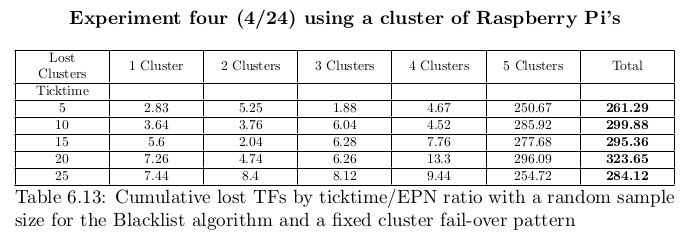
\includegraphics[scale=0.4]{./graphics/res4.png}
	}
	\frame{
		\frametitle{Experiments}
		\framesubtitle{Experiment 5}
		\begin{columns}[T]
		
		\begin{column}{0.5\textwidth}
		~\\~\\~\\
		\begin{itemize}
			\item Definition
		\end{itemize}
		Ticktime influence on the Blacklist algorithm with a random cluster fail-over pattern using a random sample size
		\end{column}
		
		\begin{column}{0.5\textwidth}
		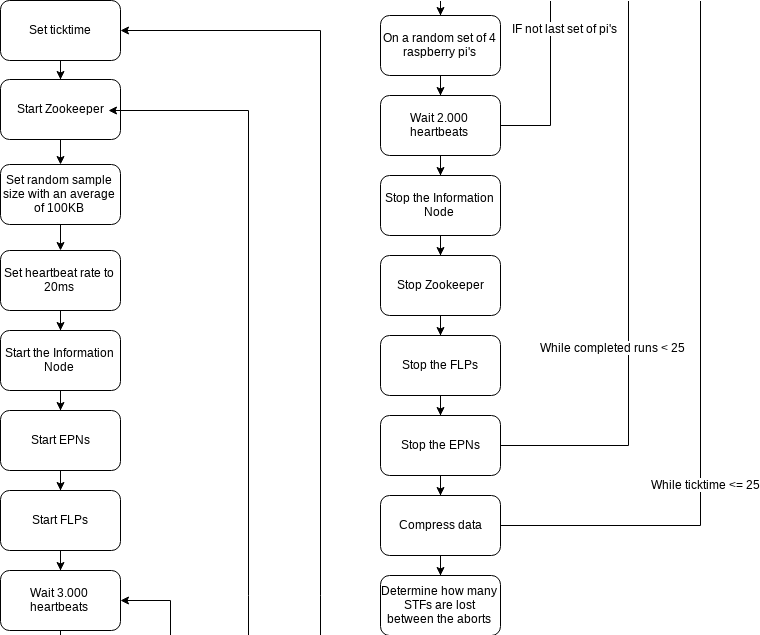
\includegraphics[scale=0.2]{./graphics/ex5.png}
		\end{column}
		
		\end{columns}
		\footnote{Effects of the EPNs and FLPs on the Information Node for ALICE (Puls, 2018, p. 26)}
	}	
	\frame{
		\frametitle{Experiment 5}
		\framesubtitle{Results}
		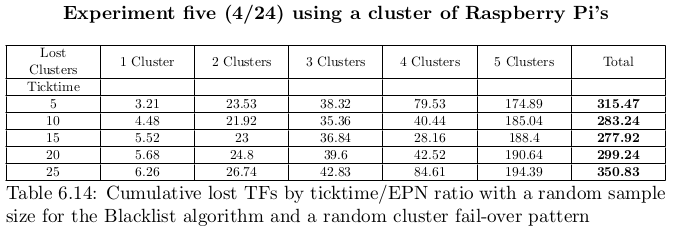
\includegraphics[scale=0.4]{./graphics/res5.png}
	}
	
	% Conclusions
	\frame{
		\frametitle{Conclusions}
		\framesubtitle{Compare}
		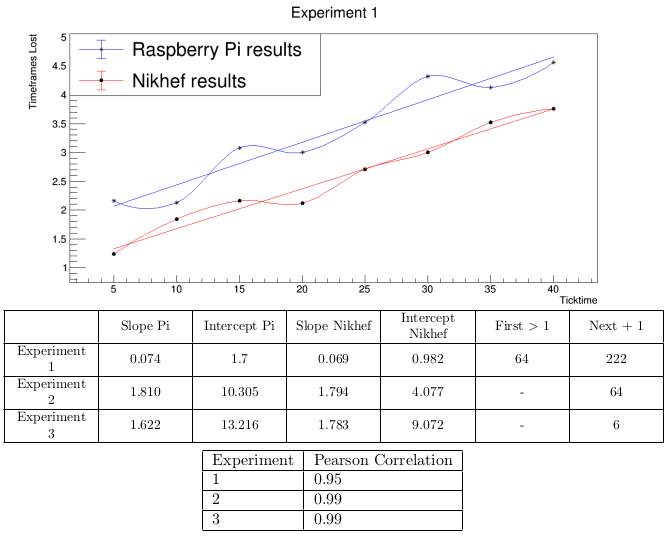
\includegraphics[scale=0.4]{./graphics/compare.png}
	}
	\frame{
		\frametitle{Conclusions}
		\framesubtitle{Expand 2 -$>$ 3}
		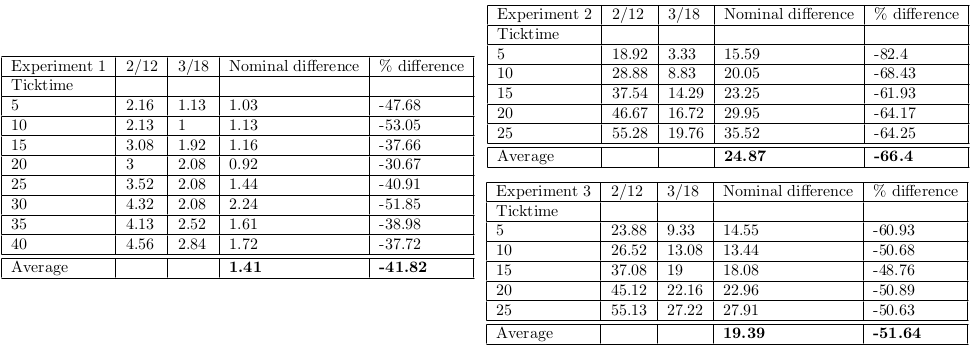
\includegraphics[scale=0.3]{./graphics/expand1.png}
	}
	\frame{
		\frametitle{Conclusions}
		\framesubtitle{Expand 3 -$>$ 4}
		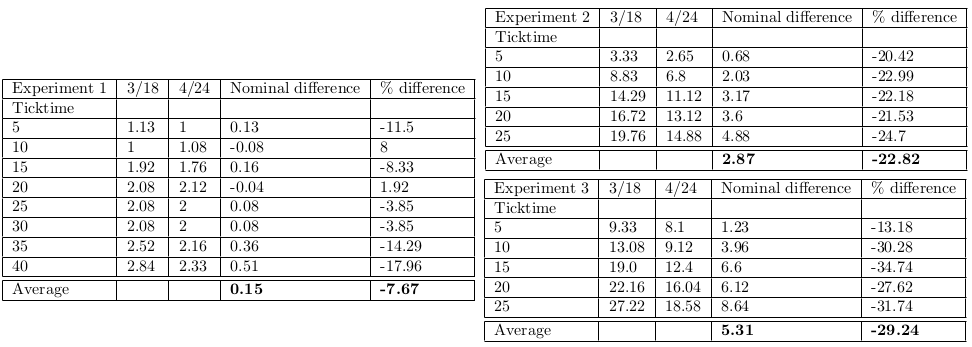
\includegraphics[scale=0.3]{./graphics/expand2.png}
	}
	\frame{
		\frametitle{Conclusions}
		\framesubtitle{Cluster fail-over}
		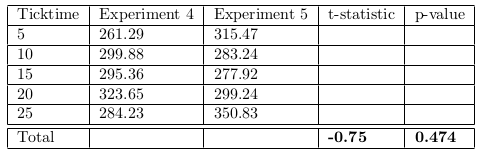
\includegraphics[scale=0.6]{./graphics/ttest.png}
	}
	
	%Discussion
	\frame{
		\begin{center}
		\frametitle{Recommendations}
		\textbf{1. Increase the unit count even further}\\~\\
		\textbf{2. Do the experiment with Ansible induced fail-overs}\\~\\
		\textbf{3. Use a lowest latency approach, as opposed to a round robin for the distribution}
		\end{center}
	}
	
	% THE END
	\frame{
		\frametitle{The end}
		\subtitle{Any questions?}
		\maketitle
	}
\end{document}